\documentclass{standalone}
\usepackage{tikz}
\begin{document}
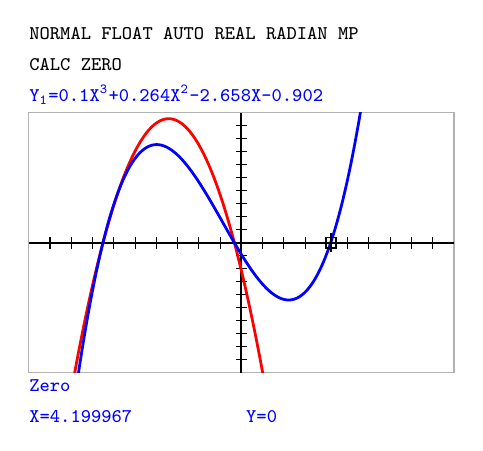
\begin{tikzpicture}[color=black, >=stealth, x=0.27cm, y=0.165cm]
  % Calculator screen (TI-84 CALC ZERO), window [-10,10] x [-10,10], ticks every 1
  \node[anchor=south west, font=\ttfamily\scriptsize, inner sep=0pt] at (-10,15.6)
    {NORMAL FLOAT AUTO REAL RADIAN MP};
  \node[anchor=south west, font=\ttfamily\scriptsize, inner sep=0pt] at (-10,13.2)
    {CALC ZERO};
  \node[anchor=south west, font=\ttfamily\scriptsize, inner sep=0pt, blue] at (-10,10.6)
    {Y\textsubscript{1}=0.1X\textsuperscript{3}+0.264X\textsuperscript{2}-2.658X-0.902};
  % Graph window border
  \draw[gray!60] (-10,-10) rectangle (10,10);
  % Axes and unit tick marks
  \draw[thick] (-10,0) -- (10,0);
  \draw[thick] (0,-10) -- (0,10);
  \foreach \t in {-9,...,-1,1,2,...,9} {
    \draw (\t,-0.45) -- (\t,0.45);
    \draw (-0.25,\t) -- (0.25,\t);
  }
  \begin{scope}
    \clip (-10,-10) rectangle (10,10);
    % Red parabola: numerator of r(x) from question 1B.B.11 (not shown on screen)
    \draw[red, line width=1pt, smooth, samples=150, domain=-8:1.3]
      plot (\x, {-\x*\x - 6.84*\x - 2.148});
    % Blue cubic Y1 = 0.1x^3 + 0.264x^2 - 2.658x - 0.902
    \draw[blue, line width=1pt, smooth, samples=200, domain=-8:6.2]
      plot (\x, {0.1*\x*\x*\x + 0.264*\x*\x - 2.658*\x - 0.902});
  \end{scope}
  % Trace cursor at the zero X = 4.199967
  \draw[line width=0.8pt] (4.2,-0.75) -- (4.2,0.75);
  \draw[line width=0.8pt] (3.85,0) -- (4.55,0);
  \draw[line width=0.6pt] (3.95,-0.4) rectangle (4.45,0.4);
  % Result readout
  \node[anchor=north west, font=\ttfamily\scriptsize, inner sep=0pt, blue] at (-10,-10.5)
    {Zero};
  \node[anchor=north west, font=\ttfamily\scriptsize, inner sep=0pt, blue] at (-10,-12.9)
    {X=4.199967};
  \node[anchor=north west, font=\ttfamily\scriptsize, inner sep=0pt, blue] at (0.2,-12.9)
    {Y=0};
\end{tikzpicture}
\end{document}
